\documentclass[10pt]{article}

\usepackage[utf8]{inputenc}
\usepackage[spanish]{babel}

\usepackage{graphicx}
\usepackage[shortlabels]{enumitem}
\usepackage{url}
\usepackage{hyperref}
\usepackage[margin=1in]{geometry}
\usepackage{here}

\newcommand{\subsubsubsection}[1]{\paragraph{#1}\mbox{}\\}
\setcounter{secnumdepth}{4}
\setcounter{tocdepth}{4}


\title{
    \vspace{-2cm}
    
\includegraphics[width=0.2 \linewidth]{Logos/UIS.pdf} \\
    Documento complementario: \\ Proyecto final dirección empresarial 2020-2.}
\author{Valentina Galvis Bergsneider \\ 
    Daniel David Delgado Cervantes \\ 
    Gianfranco Estevez Ruiz \\ 
    Equipo \# 9
    Big Ideas
}

\begin{document}

    \maketitle

\section{Items a cumplir}

\begin{enumerate}[a)]
    \item Nombre empresa: Big Ideas
    \item Logo: visible en todas nuestras redes. [\textit{\href{https://www.instagram.com/bigideasde1/}{Instagram}, \href{https://vvisgal2.wixsite.com/bigideas/}{Página web}}]
    \item Descripción logo: Nuestra empresa se dedica a la elaboración de ideas creativas para nuestros clientes en pro de lograr los objetivos buscados en su empresa. Como muestra nuestro logro siempre estamos a favor del trabajo en equipo.
    \item Eslogan: Visible en la bio de nuestra página de [\textit{\href{https://www.instagram.com/bigideasde1/}{Instagram}}]. 
    \item Misión: Presente en nuestra [\textit{\href{https://vvisgal2.wixsite.com/bigideas/}{Página web}}]. Visible más abajo de nuestros objetivos.
    \item Objetivos: Presentes en nuestra [\textit{\href{https://vvisgal2.wixsite.com/bigideas/}{Página web}}]. Visible debajo de la descripción de nuestra empresa.
    \item Estructura organizacional: Desarrollado en \url{draw.io}. Disponible [\textit{\href{https://drive.google.com/file/d/1GQhwDbZ2K-pRW-nCA6m8geqAIBCA47fB/view?usp=sharing}{aquí}}].
    \item Portafolio: Nuestro portafolio está presente en su respectiva sección en nuestra [\textit{\href{https://vvisgal2.wixsite.com/bigideas/}{Página web}}]. 
    \item Cargos y perfiles: Disponibles en nuestra [\textit{\href{https://vvisgal2.wixsite.com/bigideas/}{Página web}}] después de nuestro portafolio de servicios.
    \item Entrevistas: Disponibles en cerca del final de [\textit{\href{https://vvisgal2.wixsite.com/bigideas/}{Página web}}]. Enlaces directos: [\textit{\href{https://vvisgal2.wixsite.com/bigideas/?wix-vod-video-id=aa3ba8c458cb47f881184501249f95c5&wix-vod-comp-id=comp-klimkz5b}{Entrevista 1}}], [\textit{\href{https://vvisgal2.wixsite.com/bigideas/?wix-vod-video-id=1f5426ba028f469e897903d3fca578a6&wix-vod-comp-id=comp-klimkz5b}{Entrevista 2}}], [\textit{\href{https://vvisgal2.wixsite.com/bigideas/?wix-vod-video-id=f705a2bd32fa4610a66c9a06e5741391&wix-vod-comp-id=comp-klimkz5b}{Entrevista 3}}].
    \item Elementos audiovisuales: Los elementos audiovisuales pueden ser principalmente vistos en nuestra página de [\textit{\href{https://www.instagram.com/bigideasde1/}{Instagram}}] en las publicaciones. Estos también están presentes en nuestra [\textit{\href{https://vvisgal2.wixsite.com/bigideas/}{Página web}}].
    \item Promoción de la empresa: Esto se dió principalmente a través de [\textit{\href{https://www.instagram.com/bigideasde1/}{Instagram}}] y nuestra [\textit{\href{https://vvisgal2.wixsite.com/bigideas/}{Página web}}].
\end{enumerate}

\section{Conclusión}

Este trabajo fue muy útil para mejorar el trabajo en equipo y el compromiso por parte de cada integrante. También, fue muy interesante ver como comienza un sueño y se hace realidad (Dando alusión a las personas cuando crean sus verdaderas empresas). Tuvimos que analizar y aprender de empresas asesoras reales para darle más realismo al trabajo.

\section{Propuesta de mejora}

Sería muy interesante tener que llenar los formatos legales (RUT, RUES, DIAN, Registro mercantil, etc). No de una forma real pero si tal vez basado en una imagen editarla para llenar el formulario y así tener un “portafolio” de los documentos legales de la empresa.

\section{Evidencia reuniones}

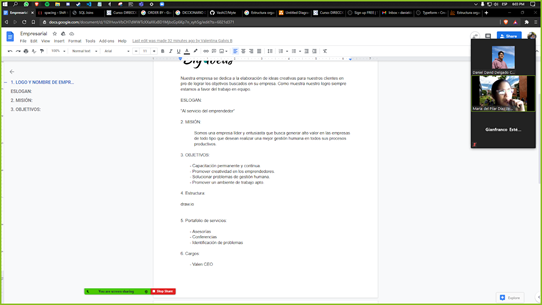
\includegraphics[width=0.75 \linewidth]{Logos/Picture1.png}

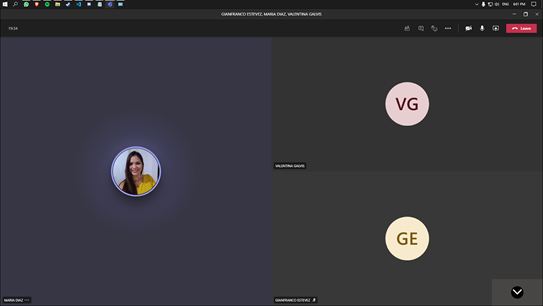
\includegraphics[width=0.75 \linewidth]{Logos/Picture2.png}

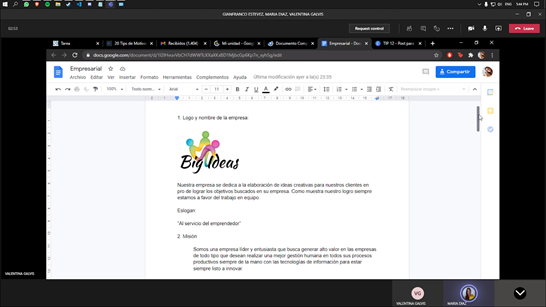
\includegraphics[width=0.75 \linewidth]{Logos/Picture3.png}

\end{document}